
\begin{frame}
	\frametitle{About Matplotlib}

    \begin{itemize}
    \item Python-based, open-source plotting library
    \item Available for all Python installations for different operating systems
    \item Uses data structures from other Python libraries like NumPy
    \item Integrates well with Python scientific libraries (NumPy, SciPy,...)
    \item Together with these libraries provides Matlab-like functionality 
    \item Access to Python file processing functions for convenient, cross-platform data handling 
    \item Can by used interactively in environments like Jupyter or in batch mode
    \item Plots can be saved in various file formats including PNG bitmap and PDF vector graphics
    \end{itemize}

\end{frame}

\begin{frame}
	\frametitle{Installation}
    \begin{itemize}
      \item For Windows and macOS:		
      \item Anaconda Python: https://www.anaconda.com/products/individual
			\item If not included: \kommandozeile{conda install -c conda-forge matplotlib}      
      \item Linux variants:
      \item Use package manager to install python
			\item Use pip to install matplotlib: \kommandozeile{pip install -U matplotlib}
			\item Use Jupyter online to try it online: https://jupyter.org/try
			\item Anaconda install Jupyter Windows/macOS: \kommandozeile{conda install ipython jupyter}
			\item Pip install Jupyter: \kommandozeile{pip install --upgrade ipython jupyter}
    \end{itemize}
\end{frame}

\begin{frame}
    \begin{center}
      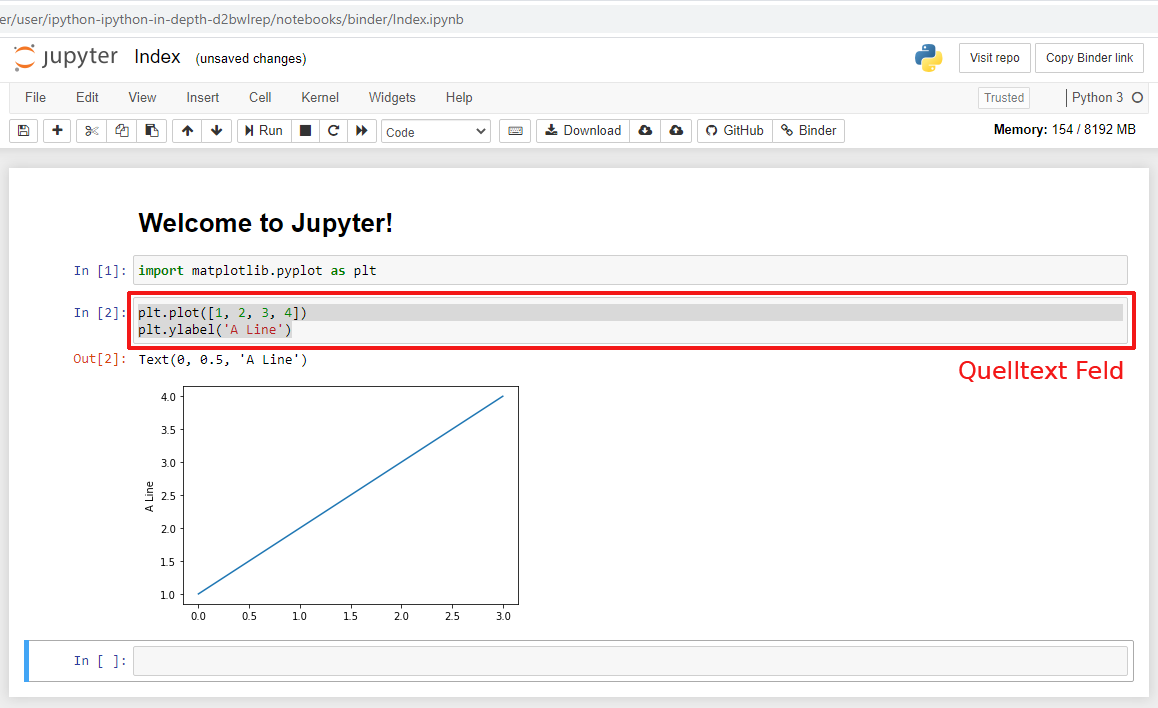
\includegraphics[width=0.9\textwidth]{screenshots/jupyter-1.png}
    \end{center}		
\end{frame}

\begin{frame}
	\frametitle{Start a Juypter Notebook}
    \begin{itemize}
      \item Command line, Terminal or CMD: \kommandozeile{jupyter notebook}
      \item Runs in browser window
			\item In Visual Studio Code: 
			\item \keyword{STRG + SHIFT + P->Jupyter: Create New Blank Jupyter Notebook} 			
    \end{itemize}
    \begin{center}
      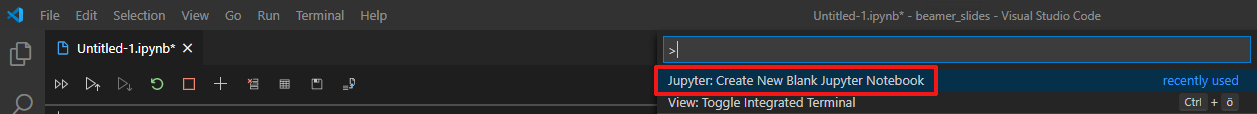
\includegraphics[width=1.0\textwidth]{screenshots/vsc-2.png}
    \end{center}				
\end{frame}

\begin{frame}
    \begin{center}
      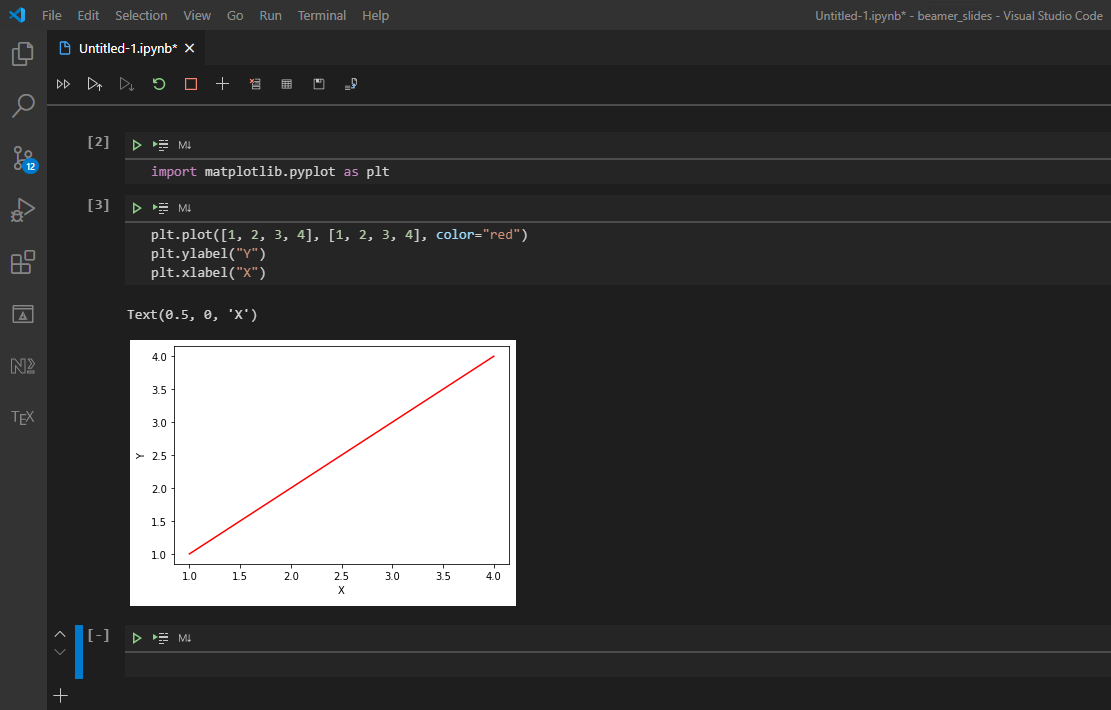
\includegraphics[width=0.9\textwidth]{screenshots/vsc-1.png}
    \end{center}				
\end{frame}

\begin{frame}[fragile]
	\frametitle{Matplotlib from the Command Line}
    \begin{itemize}
      \item Create a file \keyword{my-first-plot.py}
    \end{itemize}
    \begin{block}{File: my-first-plot.py}
    \begin{lstlisting}[language=Python]
    import matplotlib.pyplot as plt
    plt.plot([1,2,3,4], [1, 4, 9, 16], color="red")
    plt.show()
    \end{lstlisting}      
		\end{block}		
    \begin{itemize}
      \item Run the python script \keyword{python ./my-first-plot.py}
    \end{itemize}			
    \begin{center}
      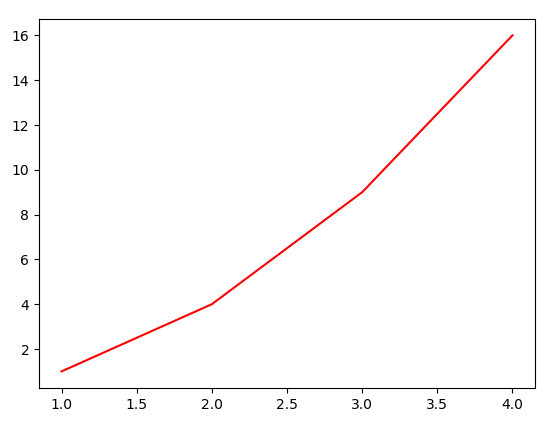
\includegraphics[width=0.25\textwidth]{screenshots/plt-2.png}
    \end{center}						
\end{frame}

\begin{frame}[fragile]
   \vspace{-1cm}
    \begin{center}
      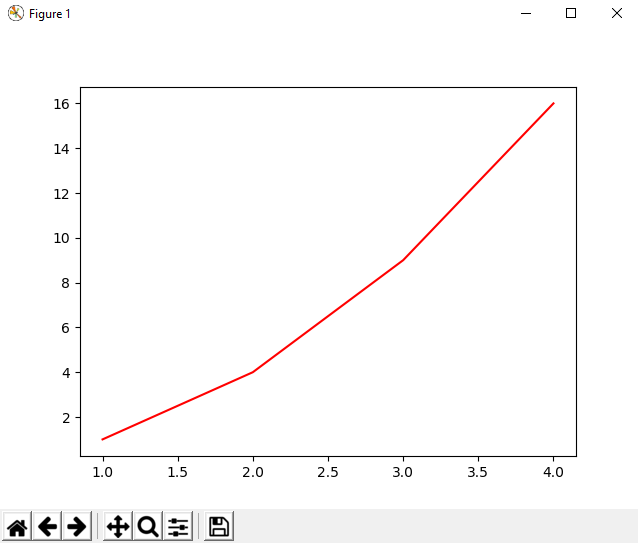
\includegraphics[width=0.7\textwidth]{screenshots/plt-1.png}
    \end{center}						
\end{frame}

\begin{frame}[fragile]
	\frametitle{Matplotlib from the Command Line}
    \begin{itemize}
      \item Create a file \keyword{my-first-plot.py}
    \end{itemize}
    \begin{block}{File: my-first-plot.py}
    \begin{lstlisting}[language=Python]
    import matplotlib.pyplot as plt
    plt.plot([1,2,3,4], [1, 4, 9, 16], color="red")
    plt.show()
    \end{lstlisting}      
		\end{block}		
    \begin{itemize}
      \item Run the python script \keyword{python ./my-first-plot.py}
    \end{itemize}			
\end{frame}